\documentclass{article}

\usepackage{array}
\usepackage{tikz}

\usetikzlibrary{shapes.multipart}
\usetikzlibrary{shapes.geometric}
\usetikzlibrary{arrows.meta}
\usetikzlibrary{positioning}
\usetikzlibrary{calc}

\usepackage[normalem]{ulem}

\tikzset{%
    pics/entity/.style n args={3}{code={%
        \node[draw,
        rectangle split,
        rectangle split parts=2,
        text height=1.5ex,
        ] (#1)
        {#2 \nodepart{second}
            \begin{tabular}{>{\raggedright\arraybackslash}p{8.5em}}
                #3
            \end{tabular}
        };%
    }},
    pics/weakentity/.style n args={3}{code={%
        \node[draw,
        rectangle split,
        rectangle split parts=2,
        text height=1.5ex,
        double,
        double distance = 0.07cm,
        ] (#1)
        {#2 \nodepart{second}
            \begin{tabular}{>{\raggedright\arraybackslash}p{8.5em}}
                #3
            \end{tabular}
        };%
    }},
    pics/relattribute/.style n args={2}{code={%
        \node[draw,
        text height=1.5ex,
        ] (#1)
        {#2};%
    }},
    pics/relationship/.style n args={2}{code={
        \node[draw,
        diamond,
        aspect=2,
        align=center,
        text height=1.5ex,
        ] (#1)
        {#2};%
    }},
    pics/defrelationship/.style n args={2}{code={
        \node[draw,
        diamond,
        aspect=2,
        align=center,
        text height=1.5ex,
        double,
        double distance = 0.07cm,
        ] (#1)
        {#2};%
    }},
    zig zag to/.style={% lines between entities and relationships
        to path={(\tikztostart) -| ($(\tikztostart)!#1!(\tikztotarget)$) |-
        (\tikztotarget)}
    },
    zig zag to/.default=0.5,
    one line/.style={% generic line
        zig zag to
    },
    one line arrow/.style={% generic line with an arrow at one end
        -{Straight Barb[scale=2]}, zig zag to
    },
    double line/.style={% for total participation (double lines)
        zig zag to, double, double distance = 0.07cm
    },
    double line arrow/.style={% for total participation, with an arrow
        -{Straight Barb[scale=0.7]}, zig zag to, double,
        double distance = 0.07cm
    },
    dashed line/.style={% for relationship attributes
        zig zag to, dashed
    },
    specialization/.style={% for specialization
        -{Latex[round,open,scale=2]}, zig zag to
    }
}
\begin{document}
    \begin{center}
        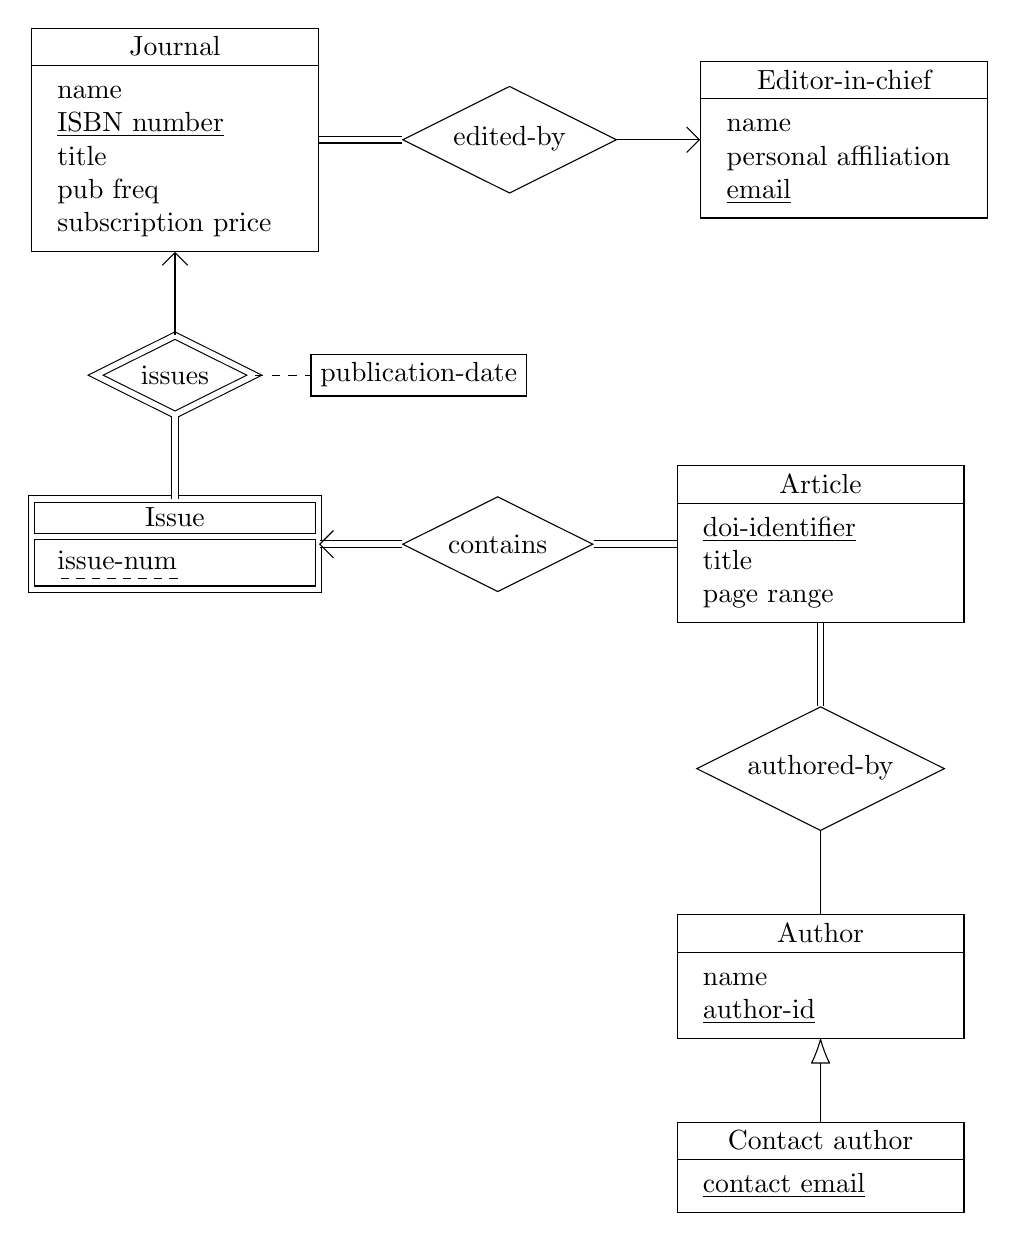
\begin{tikzpicture}
            \pic {entity={140358354984912}{Journal}{%
                name\\
                \underline{ISBN number}\\
                title\\
                pub freq\\
                subscription price\\
            }};
            \pic[right=3em of 140358354984912] {relationship={140358391825792}{edited-by}};
            \pic[right=3em of 140358391825792] {entity={140358354984816}{Editor-in-chief}{%
                name\\
                personal affiliation\\
                \underline{email}\\
            }};
            \draw[double line] (140358391825792.west) -- (140358354984912.east);
            \draw[one line arrow] (140358391825792.east) -- (140358354984816.west);
            \pic[below=3em of 140358354984912] {defrelationship={140358391825792}{issues}};
            \pic[below=3em of 140358391825792] {weakentity={140358354984768}{Issue}{%
                \dashuline{issue-num}\\
            }};
            \draw[one line arrow] (140358391825792.north) -- (140358354984912.south);
            \draw[double line] (140358391825792.south) -- (140358354984768.north);
            \pic[right=2em of 140358391825792] {relattribute={a140358391825792}{%
                publication-date
            }};
            \draw[dashed line] (140358391825792.east) -- (a140358391825792.west);
            \pic[right=3em of 140358354984768] {relationship={140358391825792}{contains}};
            \pic[right=3em of 140358391825792] {entity={140358355262528}{Article}{%
                \underline{doi-identifier}\\
                title\\
                page range\\
            }};
            \draw[double line arrow] (140358391825792.west) -- (140358354984768.east);
            \draw[double line] (140358391825792.east) -- (140358355262528.west);
            \pic[below=3em of 140358355262528] {relationship={140358391825792}{authored-by}};
            \pic[below=3em of 140358391825792] {entity={140358355262912}{Author}{%
                name\\
                \underline{author-id}\\
            }};
            \draw[double line] (140358391825792.north) -- (140358355262528.south);
            \draw[one line] (140358391825792.south) -- (140358355262912.north);
            \pic[below=3em of 140358355262912] {entity={140358391825936}{Contact author}{%
                \underline{contact email}\\
            }};
            \draw[specialization] (140358391825936.north) -- (140358355262912.south);
        \end{tikzpicture}
    \end{center}
\end{document}
